\chapter[Teoretická část práce]{Teoretická část práce}

\section{Hardwarové vybavení}

\subsection*{Raspberry Pi}
Raspberry Pi je název malého, jednodeskového počítače vyvinutého britskou nadací Raspberry Pi Foundation v roce 2012 s cílem podpořit výuku informatiky a vytvořit počítač dostupný pro všechny. V roce 2017 byla dostupná již třetí generace tohoto minipočítače a také zmenšená verze Raspberry Pi Zero a Zero W.

Primárním operačním systémem je Raspbian, což je derivát Linuxu Debianu, avšak je možné použít i řadu jiných operačních systémů, například Windows IoT Core nebo RISC OS.\cite{rpidoc}

\subsubsection{Raspberry Pi Zero W}
Základem Raspberry Pi Zero W je SoC (System on a chip) Broadcom BCM2835 založený na 32 bitové architektuře ARMv6. Taktovací frekvence procesoru je 1 GHz.

Počítač je vybaven 512 MB paměti typu SDRAM a grafickým procesorem Broadcom Videocore IV. Pro úložiště dat jsou použity microSD karty.

Doporučená cena v době uvedení na trh byla 10 USD.\cite{rpidoc}

\begin{figure}[h]
  \begin{center}
    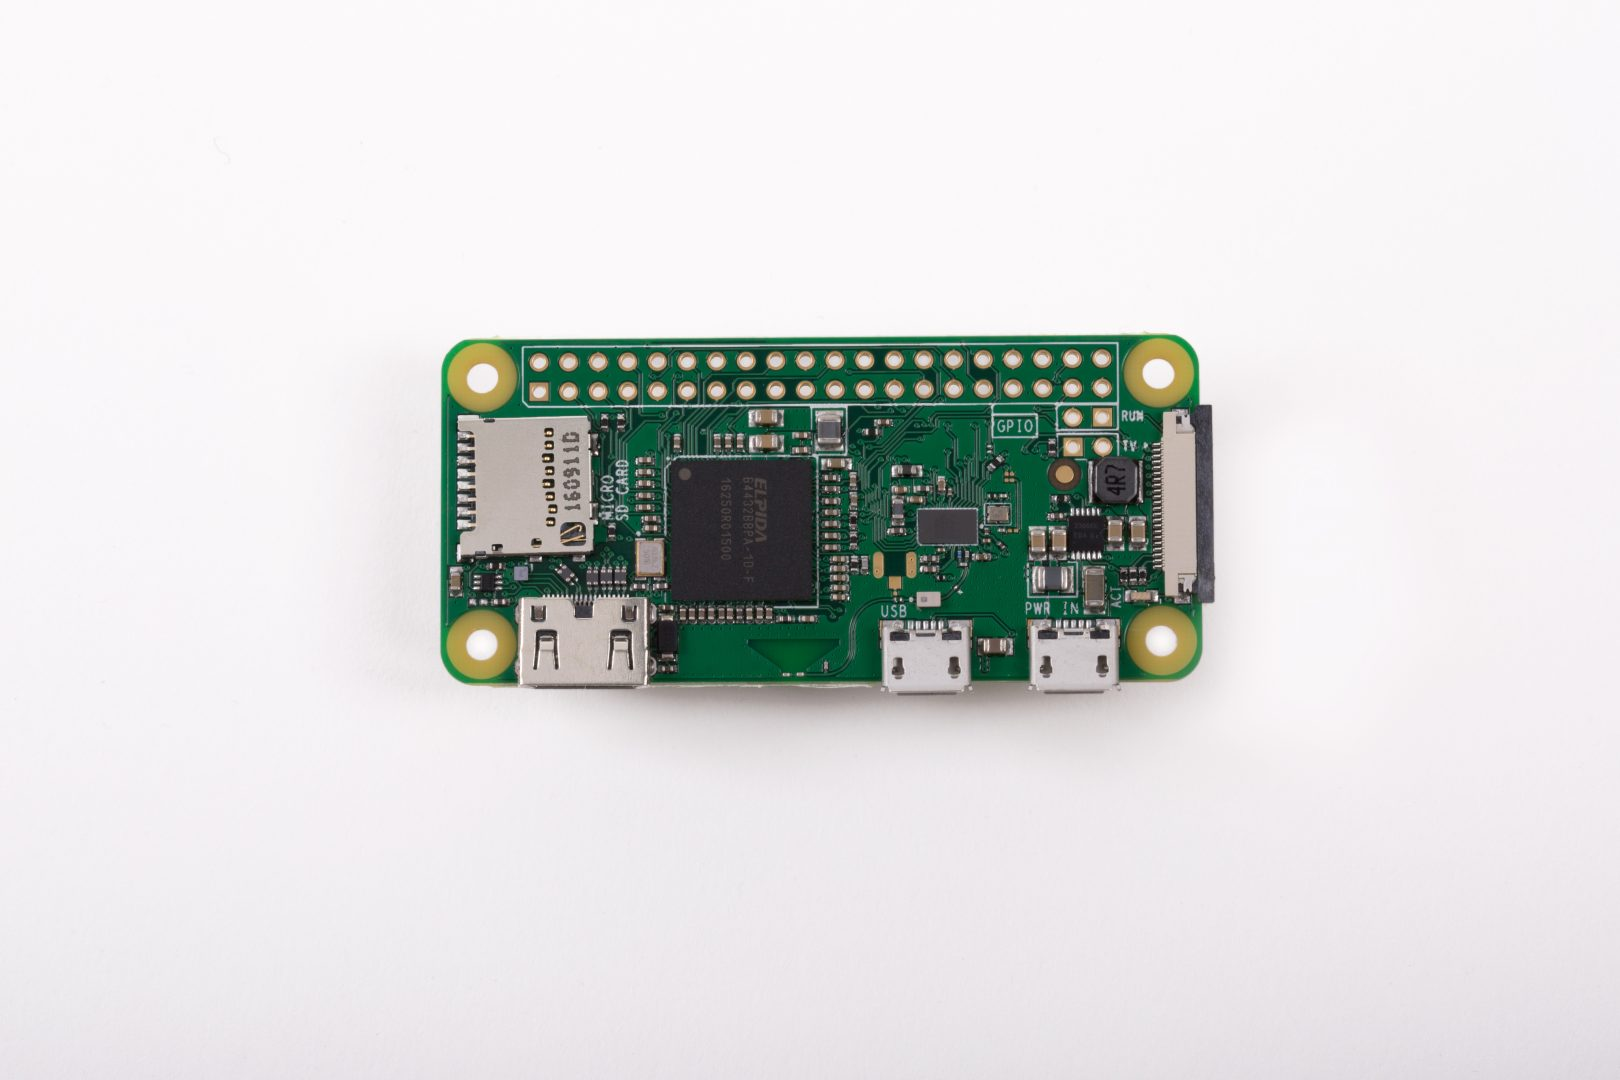
\includegraphics[scale=0.3]{obrazky/rpizero.jpg}
  \end{center}
  \caption{Raspberry Pi Zero W, převzato z thepihut.com}
\end{figure}

\subsubsection{Napájení a spotřeba}
Zařízení je napájeno z micro USB portu napájecím napětím 5V. Dle technické dokumentace se proudový odběr ve stavu nečinnosti pohybuje kolem 100 mA. Maximální odběr zařízení včetně zapojené klávesnice, myši a obrazovky může být až 350 mA.

Nicméně lze různými postupy snížit proudový odběr až na 80 mA ve stavu nečinnosti. Například vypnutím HDMI portu se odběr sníží o 25 mA, vypnutí LED diod ušetří až 5 mA.
Spotřeba elektrické energie také velmi záleží na počtu připojených perifierií. Samostatná Python kamera má spotřebu přibližně 250 mA.

Velký vliv na spotřebu má také vytížení procesoru.
Bude tedy vhodné optimalizovat algoritmus detekce obrazu tak, aby využíval co nejméně procesorového času a ve výsledku spotřeboval co nejméně elektrické energie.

\subsubsection{GPIO}
GPIO je zkratka pro General Purpose Input Output. Jsou to uživatelsky konfigurovatelné piny, které mohou být jak vstupní, tak výstupní. Raspberry Pi Zero, Raspberry Pi 3 a Raspberry Pi 2 disponuje 40 takovými piny. Pro srovnání - první verze Raspberry Pi A a B disponovala pouze 26 těmito piny.

Raspberry Pi používá 3,3voltovou logiku, je tedy nutné použít pro zapojení periferií využívajících 5 V převodník úrovní.

GPIO je možné nastavit například jako UART, SPI, I2C nebo PCM.

Pro ovládání GPIO lze použít Python modul GPIO, který ale v době psaní práce (verze 0.63) umožnil pouze softwarové GPIO. Nebylo tedy například umožněno hardwarové generování PWM signálu.

Pro hardwarové generování signálu lze využít modul RPIO, který umožňuje generování PWM pomocí DMA s přesností 1,2 mikrosekundy.

\begin{figure}[!h]
  \begin{center}
    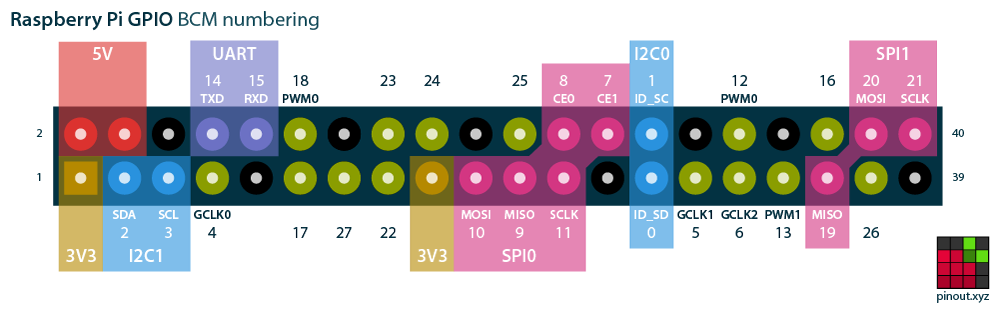
\includegraphics[scale=0.41]{obrazky/raspberry-pi-pinout.png}
  \end{center}
  \caption{Raspberry Pi GPIO Pinout, převzato z pinout.xyz}
\end{figure}

\subsubsection{Úložiště}
Raspberry Pi standardně používá jako úložiště (micro)SD karty. Maximální propustnost čtečky karet je 25 MB/s, je dána omezením sběrnice USB.

Spotřebitelské SD karty používají levné paměti typu TLC. Berme tedy v úvahu, že spotřebitelské SD karty mají kratší životnost než při užití pevného disku. K dostání jsou ale i karty pro průmyslové použití, které využívají pamětí typu MLC či SLC, které mají několikanásobně vyšší životnost než TLC paměti.

Životnost paměti se dá zvýšit například použitím RAM disku tmpfs v Linuxu. Také je možné přesunout root na jiný typ úložiště a SD kartu ponechat pouze na bootování.

Při preferenci co nejnižší spotřeby elektrické energie monitorovacího zařízení, bude vhodné použít jako hlavní datové úložiště pouze SD kartu.

\subsection*{Raspberry Pi NoIR Camera Board V2}
Vzhledem k požadavku na noční snímání je použita kamera bez infračerveného filtru Raspberry Pi NoIR Camera Board V2. Kvůli absenci IR filtru je možné využití okem neviditelného infračerveného přísvitu.

\begin{figure}[h]
  \begin{center}
    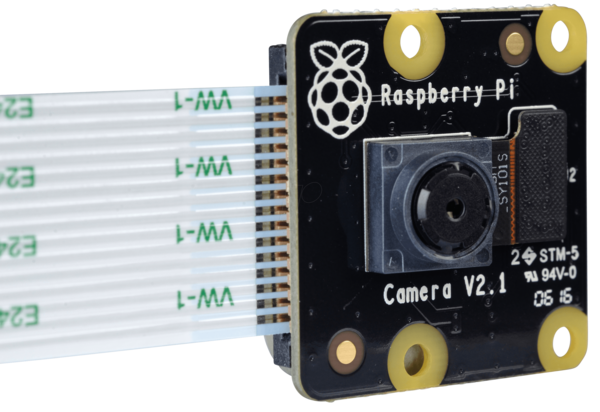
\includegraphics[scale=0.3]{obrazky/rpicamera.png}
  \end{center}
  \caption{Raspberry Pi NoIR Camera V2, převzato z reichelt.de}
\end{figure}

Kamera disponuje 8 megapixelovým obrazovým senzorem Sony IMX219 a fixním ohniskem. Videa je možné natáčet až do rozlišení 1920x1080 pixelů při 30 fps a je možné pořizovat statické snímky až do rozlišení 3820x2464 pixelů.

Zorné pole kamery v horizontálním směru je 62 úhlových stupňů.

Kamera je připojena pomocí vysokorychlostního sériového rozhraní CSI, které má ve verzi 3 teoretickou maximální datovou propustnost 5,8 Gbps.

\begin{figure}[!h]
  \begin{center}
    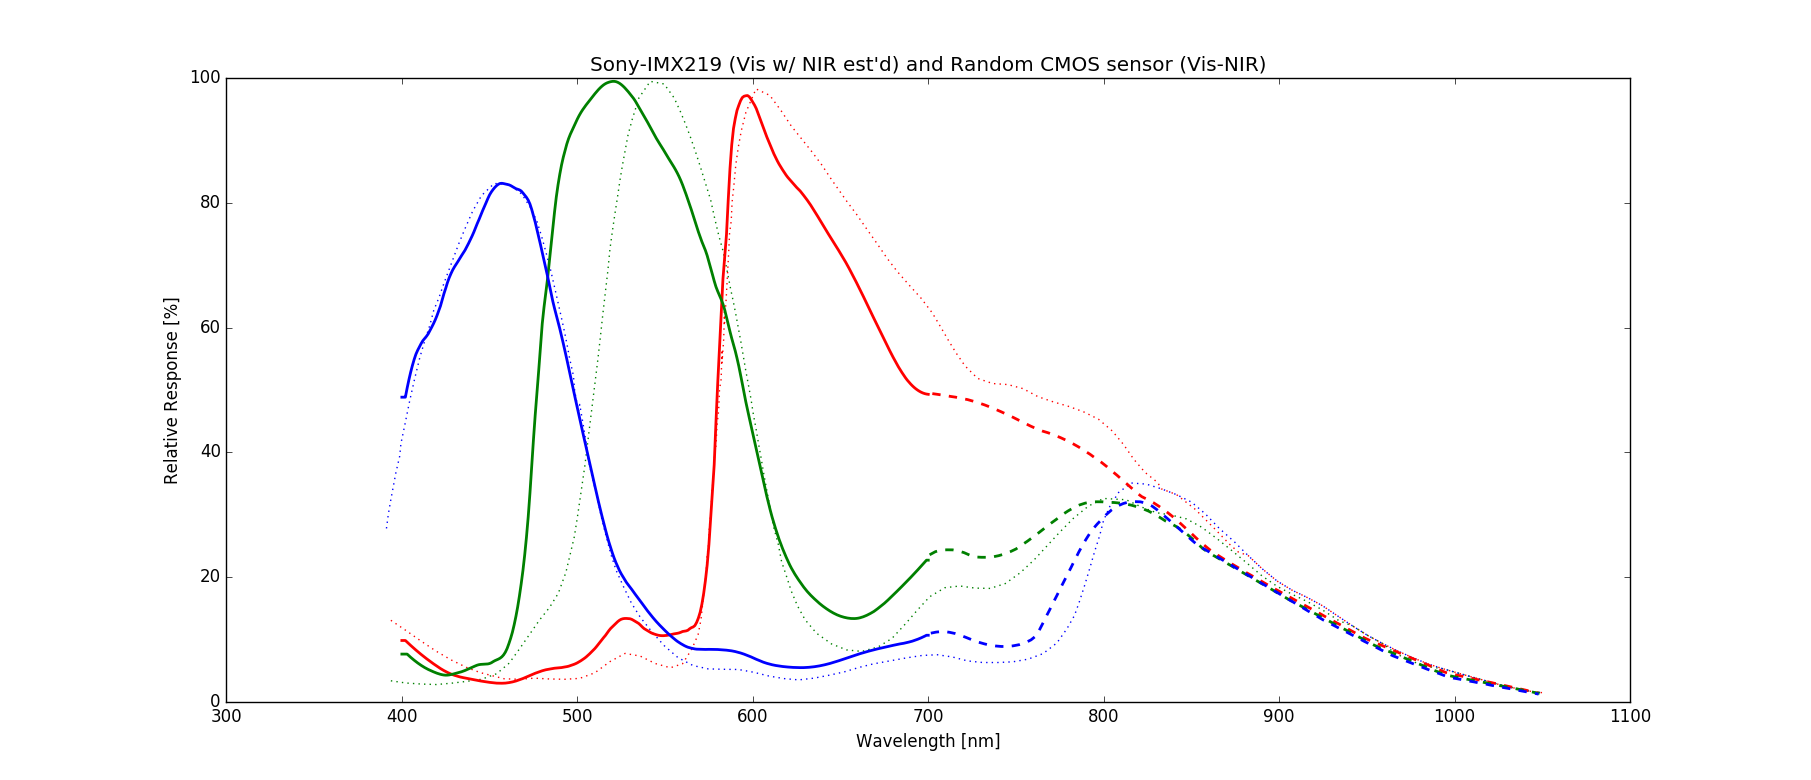
\includegraphics[scale=0.32]{obrazky/SonyIMX219approx.png}
  \end{center}
  \caption{Aproximovaná spektrální citlivost CMOS snímače Sony IMX219. Autorem je Koen Hufkensem  \cite{sony}}
\end{figure} 
Data zobrazena plnou čarou zobrazují spektrální citlivost ve viditelném spektru a jsou extrahovány z datasheetu produktu.

Data zobrazena přerušovanou čarou jsou aproximována porovnáním spektrální citlivosti podobného CMOS snímače od firmy Sony.

Z grafu tedy vyplývá, že citlivost snímače klesá se prodlužující se vlnovou délku světla, které dopadá na snímač CMOS. Přibližně při vlnové délce světla 1050 nm je spektrální citlivost snímače rovna téměř nulová.

Tuto informaci můžeme využít k nákupu vhodné infračervené diody pro přísvit kamery, aby bylo zajištěno dobré snímání obrazu při nevhodných světelných podmínkách.

\subsection*{GSM/GPRS modul SIM800}
SIM800 je modul od společnosti SIMCom pro bezdrátovou komunikaci pomocí technologie GSM a GPRS.

Podporuje frekvenční pásma 850/900/1800/1900 MHz, hlasovou komunikaci, SMS a GPRS data třídy 10.

Maximální teoretická přenosová rychlost pro CS4 je tedy 85,6 kbps pro downlink a 21,4 kbps pro uplink. Ke komunikaci je možné využít sériové rozhraní podporující AT příkazy, nebo je možné využít PPP stack pro internetové připojení.

Pro připojení k Raspberry Pi využijeme sériovou sběrnici UART. Modul podporuje baudovou rychlost od 1200 do 460800 Bd. 

\subsubsection{Point-to-Point Protocol}
Point-to-Point Protocol, zkráceně PPP je název komunikačního protokolu linkové vrstvy, používaný pro přímé spojení mezi dvěma síťovými uzly.

V našem případě budeme tento protokol používat pro navázání spojení mezi GPRS modulem po sériové lince. K připojení je použit program PPPD, který naváže spojení pomocí tzv. chatovacích skriptů.

\subsubsection{AT příkazy}
AT příkazy jsou instrukce pro řízení modemu. AT je zkratka pro ATention.

Každý příkaz začíná "AT". Jako příklad uveďme příkazy specifické pro komunikaci s GSM/GPRS modemem: AT+CMGS je příkaz pro odesílání SMS zprávy, AT+CGSN je příkaz pro získání IMEI čísla modemu.

\subsubsection{APN}
APN, neboli Access Point Name je jméno brány mezi sítí GSM/GPRS a sítí Internet. Název APN pro daného mobilního operátora nám musí být znám před připojením.

\subsection*{PIR modul HC-SR501}
Modul HC-SR501 používá PIR element LHI778 a integrovaný obvod BISS0001 pro obsluhu signálu z PIR elementu.

Modul umožňuje nastavení citlivosti snímání v rozsahu od 3 do 7 metrů vzdálenosti snímaného objektu od kamery a také nastavení časového zpoždění mezi detekovaným pohybem a odeslaným signálem o detekci.

Nastavení citlivosti snímání je prováděno pomocí potenciometru na modulu.

Napájecí napětí je v rozmezí 5 až 20 V. Pokud je detekován pohyb, objeví se na výstupním pinu logická jednička (3,3 V), která zůstane aktivní po nastavenou dobu.

Nastavení časového zpoždění je též prováděno potenciometrem.

Po vypršení nastaveného zpoždění, zůstane modul ještě 2,5 sekundy ve stavu logické nuly.

V tomto 2,5 sekundovém časovém úseku nemůže být detekován další pohyb snímaného objektu.

Modul může pracovat ve dvou režimech detekce pohybu, buď v jednoduchém nebo opakovaném.

V jednoduchém režimu dojde k zahájení odpočítávání časovače zpoždění ihned po detekci pohybu. K dalšímu restartování může dojít až po vypršení nastaveného času.

V opakovaném režimu je časovač restartován s každým dalším detekovaným pohybem.

\begin{table}[h]
\centering
\caption{Možnosti modulu HC-SR501}
\label{HC-SR501}
\begin{tabular}{|l|l|}
\hline
\textbf{Pin nebo nastavení} & \textit{Funkce}                                            \\ \hline
Zpoždění            & Jak dlouho má být na výstupním pinu logická 1                     \\ \hline
Citlivost           & Rozsah nastavení vzdálenosti od 3 m až 7 m                                   \\ \hline
Spouštění           & Jednoduché nebo opakované zpoždění.                               \\ \hline
GND                 & Uzemnění                                                          \\ \hline
Výstup              & Logický výstup 3,3 V, pokud je detekován pohyb                     \\ \hline
Napájení            & 5 až 20 V DC napětí                                                \\ \hline
\end{tabular}
\end{table}

\begin{figure}[!h]
  \begin{center}
   \begin{circuitikz} 
        \draw (0,0) node[pir] (pir) {}
            (pir.power) node[anchor=east] {Napájení}
            (pir.ground) node[anchor=east] {GND}
            (pir.out) node[anchor=east] {Výstup}
            (pir.north) node[anchor=south] {}
            (pir.south) node[anchor=north] {}
            (pir.east) node[anchor=west] {};
\end{circuitikz} 
  \end{center}
  \caption{Schéma PIR modulu}
\end{figure}


\subsection*{Výkonová IR LED dioda GT-P04IR4101}
\subsubsection{Parametry}
\begin{table}[h]
\centering
\caption{Parametry LED z katalogu}
\label{Parametry LEDl}
\begin{tabular}{|l|l|l|l|}
\hline
\textbf{Parametr}        & \textit{min.} & \textit{typická} & \textit{max.} \\ \hline
Ztrátový výkon &              & 1 W           &              \\ \hline
Úbytek napětí            & 1,65 V        &              & 1,75 V        \\ \hline
Proudový odběr            &              & 400 mA        & 420 mA             \\ \hline
Vyzářený výstupní výkon      &              & 400 mW        &              \\ \hline
Vlnová délka světla         &              & 850 nm        &              \\ \hline
Tepelný odpor         &              & 12 °C/W       &              \\ \hline
Úhel osvětlení              &              & 120°         &              \\ \hline
\end{tabular}
\end{table}

\clearpage


\section{Programové vybavení}

\subsection*{Raspbian}
Raspbian je linuxový operační systém založený na distribuci Debian. Je optimalizovaný pro hardware Raspberry Pi, určený pro architekturu armhf. První verze byla vytvořena v roce 2012. Raspbian bude použit ve verzi lite, tedy bez grafického rozhraní a pouze s nutnými programovými knihovnami - balíčky.

\subsection*{Python}
Python je vysokoúrovňový skriptovací jazyk navržený Guidem Van Rossem v roce 1991.
Jazyk podporuje několik programovacích paradigmat včetně objektového, procedurálního a funkcionálního. V roce 2017 existovaly dvě navzájem částečně nekompatibilní odnože Pythonu a to 2.7.x a 3.x.x. Python je snadno rozšířitelný o další programové knihovny - balíčky.

\subsubsection{Picamera}
Picamera je knihovna pro Python, která umožňuje ovládat kameru pro Raspberry Pi, včetně pořizování statických snímků a videí. Poskytuje poměrně bohaté programové API.

\subsubsection{Pillow}
Pillow je knihovna pro Python, která vznikla jako derivát staršího modulu PIL. Pillow rozšiřuje schopnosti Pythonu o pokročilé zpracování obrazu.

\subsubsection{PyDrive}
PyDrive je knihovna pro Python pro práci s cloudovým úložištěm Google Drive. Vznikla jako zjednodušení Google Drive REST API. Knihovna umožňuje jednoduchou manipulaci se soubory uloženými na Google Drive. K autentizaci uživatele je použit framework OAuth 2.

\subsubsection{Python-gsmmodem}
Python-gsmmodem je knihovna pro Python pro komunikaci s modemy pomocí AT příkazů. Podporuje odesílání a příjmání SMS zpráv a také hlasovou telefonii.

\subsubsection{Epsolar-tracer}
Epsolar-tracer je knihovna pro Python pro komunikaci se solárním regulátorem Epsolar využívající protokol Modbus a rozhraní RS-485. Knihovna je použita pro komunikaci mezi Raspberry Pi a solárním regulátorem.

\subsection*{Google Apps Script}
Google Apps Script je skriptovací jazyk založený na Java Scriptu pro webové aplikace běžící pod Google Cloudem. Google poskytuje běhové prostředí a editor s debuggerem. V projektu je tento jazyk využíván pro vytvoření grafického rozhraní pro konfiguraci aplikace a pro sběr dat.

\subsection*{JSON}
JSON je zkratka pro JavaScript Object Notation. Je to jednoduchý formát pro výměnu dat. Jeho výhoda spočívá v tom, že má jednoduchou strukturu. Je tedy lehce čitelný i lehce editovatelný a má také velmi dobrou podporu v programovacích jazycích. V projektu je tento formát využíván pro konfiguraci aplikace.

\subsection*{Závěr k výběru softwaru}
Veškeré vybrané softwarové vybavení se řadí do kategorie Open-source. Takový software je vyvíjen především komunitně a jeho zdrojový kód je volně k dispozici. Cena softwaru je tedy nulová.
Další kapitola se bude zabývat využitím vybraného softwaru.

\section{Detekce pohybu}
Detekce pohybu je proces detekce změny pozice zkoumaného objektu vůči pozadí. Zde se budeme zabývat především elektronickou detekcí pohybu.

Existuje několik metod elektronické detekce pohybu, například optická nebo akustická metoda. Mezi optické metody patří detekce infračerveného záření pomocí PIR senzoru. Příklad akustické metody je detekce ultrazvukem.

\subsection*{Pohyb}
Pod pojmem pohyb rozumíme pohyb mechanický, což je změna polohy pozorovaného objektu.
Pohyb nelze detekovat z jednoho statického obrazu, potřebujeme obrazový tok.
Budeme tedy pracovat s dynamickým obrazem, což je posloupnost statických obrazů.

\subsection*{Detekce pohybu pomocí PIR senzoru}
Zkratka PIR znamená „passive infrared“, jde tedy o pasivní infračervený detektor, který funguje na principu pyroelektrického jevu.

\subsection*{Pyroelektrický jev}
Pyroelektrický jev je schopnost materiálu generovat dočasný elektrický potenciál při změně teploty. Vyskytuje se u dielektrik s jednou polární osou symetrie.

\subsection*{PIR Element}
PIR element je základní funkční prvek PIR detektoru. Je to polovodičová součástka, citlivá na světlo, vyrobená ze sloučenin na bázi lithia a tantalu. PIR snímač je citlivý v širokém spektru záření, je proto nutné před snímač aplikovat filtr, který propouští pouze infračervené záření o vlnových délkách v rozsahu 8 až 14 $\jedn{\mu m}$. Lidské tělo emituje záření o vlnové délce 9,4 $\jedn{\mu m}$. Se změnou intenzity dopadajícího infračerveného záření na povrch pyroelektrického materiálu se změní hodnota elektrického povrchového náboje. Tato změna je měřena citlivým tranzistorem FET. \cite{pir_senzor}

\subsection*{Optika}
Úkolem optické soustavy je soustřeďovat infračervené záření z detekční zóny do PIR elementu. V praxi se používají Fresnelovy čočky nebo zrcadla.

\subsection*{Detekce pohybu z dynamického obrazu}
Existuje několik metod pro detekci pohybu ze snímané scény.
Metody jsou primárně založené na segmentaci pozadí a popředí obrazu.
Pozadím nazýváme část obrazu ve které zjišťujeme změny a popředí nese právě ty změny. Pozadí ale většinou nebývá statické, je v něm obsažen například šum snímacího zařízení, nebo změny osvětlení. 

Je několik algoritmů, které tyto problémy řeší s různými nároky na výpočetní výkon.

Zmiňme například:
\begin{itemize}
    \item
    Porovnávaní histogramu mezi snímky
    \item
    Sledování rozdílných bodů mezi snímky
    \item
    Porovnání snímků zpracovaných detektorem hran
    \item
    Metoda optického toku
    \item
    GMM - Gaussian Mixture Models
    \item
    Sigma-Delta filtrace
\end{itemize}

\subsection*{Porovnávání histogramu mezi snímky}
Jedná se o jednu z nejjednodušších metod detekce pohybu. Porovnávají se histogramy dvou snímků - vyhodnocují se tedy jasové charakteristiky snímků. Tato metoda je výpočetně málo náročná a je vhodná pouze do podmínek se stálým osvětlením. Je nutné dobře zvolit referenční snímek podle kterého se bude porovnávat pohyb a průběžně ho aktualizovat podle změn v prostředí. Výpočetně nejméně náročné je průměrování histogramů několika snímků, ve kterých není označen pohyb. Také je dobré snímek zbavit šumu přes šumové filtry. \cite{fbmi_video}

\subsubsection{Výhody} 
Výpočetně málo náročná metoda.
\subsubsection{Nevýhody}
Metoda je náchylná na šum a také na změny prostředí.

\subsection*{Sledování rozdílných bodů mezi snímky}
Tato metoda spočívá v porovnáváni snímků na úrovni pixelů. Je vhodné snímky nejprve převést do 8-bitového barevného prostoru a potom odečítat hodnoty.  Obrázky od sebe v této podobě odečteme a získáme nový snímek, který nyní bude prezentovat rozdíl složek. Čím méně se od sebe korespondující pixely liší, tím se jejich hodnota v rozdílu bude více blížit hodnotě 0 (černá barva). Poté je nutné aplikovat metodu prahování abychom rozeznali informaci od šumu. \cite{fbmi_video}
\subsubsection{Výhody}
Schopnost určit místo ve scéně na kterém došlo k pohybu.
\subsubsection{Nevýhody}
Relativně výpočetně náročná operace porovnávání snímků na úrovni pixelů.

\subsection*{Metoda optického toku}

Metoda optického toku dokáže sledovat pohyb pixelu mezi snímky ve video sekvenci a zjistit tak rychlost pohybu. Tímto způsobem se dá předpovídat trajektorie sledovaného objektu. Metoda je výpočetně velmi náročná pro sledování všech pixelů ve scéně. S určitou optimalizací je však použitelná i jako detektor pohybu. 

\section{Mobilní sítě}
\subsection*{GSM}
GSM (Groupe Spécial Mobile) popisuje protokoly pro mobilní telekomunikaci druhé generace. Poprvé bylo GSM použito v roce 1991 ve Finsku a následně se stalo standardem pro hlasovou komunikaci po celém světě. Standard GSM původně využíval pouze přepínání okruhů optimalizovaných pro full-duplex hlasovou telefonii, avšak příchod GPRS rozšířil síť o možnost paketového přenosu dat.

\subsection*{GPRS}
Systém GPRS (General Packet Radio Service) je rozšíření systému GPS o datový paketový přenos. Umožňuje připojení do sítě Internet.

\section{Solární napájení}
Jde o způsob získávání elektrické energie přeměnou ze sluneční energie. Energii můžeme získávat buď pomocí fotovoltaických článků, které využívají fotovoltaický jev, nebo pomocí tzv. koncentrovaných solárních panelů. Nedílnou součástí napájecího obvodu se solárními články je akumulátor, který pokrývá napájení, když článek nedodává dostatečný proud, což se děje například za zhoršených světelných podmínek nebo v noci.

\subsection*{Fotovoltaický článek}
Fotovoltaický článek využívá fotovoltaického jevu, což je jedna z forem vnitřního fotoelektrického jevu.

\subsubsection*{Princip funkce}
Fotovoltaický jev vzniká v polovodičích, když foton s dostatečnou energií uvolní elektron z valenčního pásu do pásu vodivostního. Ve valenčním pásu zůstane „chybějící elektron“, tzv. díra, kterou lze považovat za elementární kladný náboj (díra se pohybuje tak, že se do ní přemístí valenční elektron sousedního atomu, čímž se díra přesune na původní místo tohoto elektronu).

Zjednodušeně lze prohlásit, že dopadem fotonu se vytvoří pár pohyblivých nábojů elektron-díra. Tyto náboje se difúzí nebo působením elektrického pole v okolí PN přechodu pohybují ve směru k elektrodě se stejnou polaritou – elektron k záporné a díra ke kladné. Při propojení elektrod vnějším obvodem putují elektrony k opačné elektrodě, kde rekombinují s děrami – vnějším obvodem prochází elektrický proud.\cite{bechnik_2014}

\subsubsection*{Monokrystalický článek} 
Monokrystalický článek je vytvořen na jediném velkém krystalu křemíku.
Dosahuje nepatrně lepší efektivity (14 - 18 \%) než polykrystalický, a to pouze, pokud
má panel ideální orientaci ke slunci.

\subsubsection*{Polykrystalický článek}
Je složen z většího počtu článků, které jsou pak navzájem
propojeny. Panel bývá světlejší a může se na pohled jevit jako „flekatý”. Tento panel produkuje
rovnoměrnější výkon, ale má nižší účinnost (asi 12 - 17 \%). Jeho použití je vhodné, pokud budou na panel dopadat sluneční paprsky pod různým úhlem.

\subsubsection*{Efektivita solárních panelů}
Efektivita solárních panelů bude závislá především na těchto faktorech: 
\begin{itemize}
    \item Zeměpisná poloha, kde je panel umístěn.
    \item Poloha panelu vůči slunci.
    \item Velikost solárního panelu.
    \item Typ solárního panelu.
    \item Účinnost obvodu pro přenos energie. 
\end{itemize}

\begin{figure}[h]
  \begin{center}
    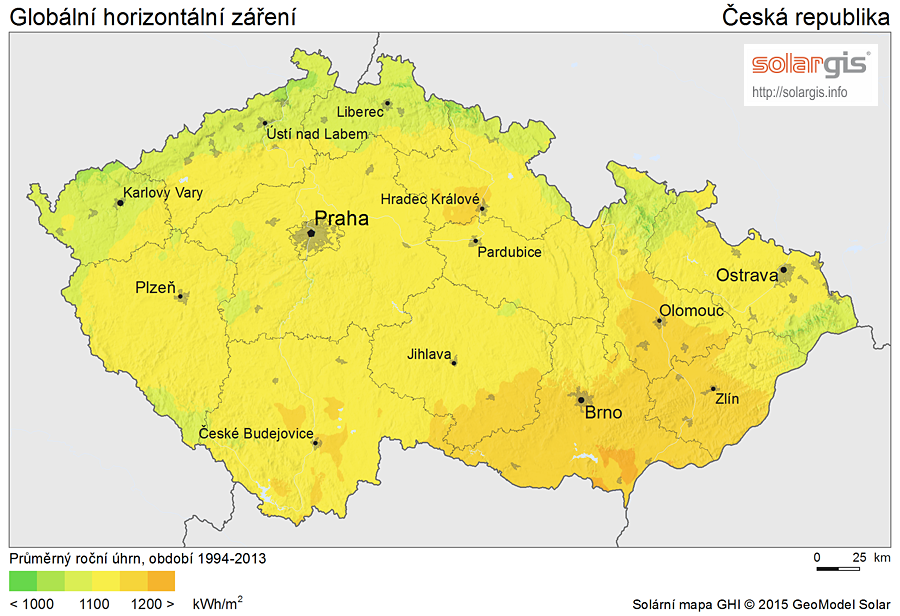
\includegraphics[scale=0.41]{obrazky/Solargis-CZ-GHI.png}
  \end{center}
  \caption{Globální horizontální záření \cite{solargis}}
\end{figure}

\subsubsection*{U solárních panelů se udávají tyto parametry:}
\begin{itemize}
\item Výkon - jaký výkon je panel schopný podávat.
\item Napětí naprázdno - jaké napětí se na svorkách panelu může objevit, pokud
není panel zatížen (spotřebičem).
\item Maximální napětí při plném výkonu - jaké napětí bude na svorkách panelu, pokud
bude zatížen maximálním povoleným proudem.
\item Maximální proud při plném výkonu - maximální povolený odebíraný protékající proud.
\end{itemize}

\subsection*{Akumulátor}
Akumulátor je zařízení, které má schopnost uchovávat energii. Nejběžnější typy elektrických akumulátorů pracují na elektrochemickém principu. Mezi takové akumulátory patří například: nikl-kadmiové (NiCd), nikl-metal hydridový (NiMh), lithium-polymerový (Li-pol), lithium-iontový (Li-ion) a olověný (Pb).

\subsection*{Lithiové akumulátory}
Lithiové akumulátory patří v současnosti k nejpoužívanějším typům akumulátorů. Najdeme je téměř v každé přenosné spotřební elektronice. 
Mezi lithiové akumulátory řadíme lithium-iontové (Li-ion) a novější lithium-polymerové (Li-pol).

Mezi výhody lithiových akumulátorů patří především velká energetická hustota, můžeme tedy mít baterii s vysokou kapacitou s relativně malou hmotností a objemem. Další výhodou je nízké samovybíjení, schopnost dodávat vysoké proudy a také relativně dlouhá životnost.

Mezi nevýhody zmiňme nutnost složitějšího obvodu pro nabíjení. Je nutné hlídat akumulátor před přílišným nabitím a vybitím a také před vysokou teplotou. Je zde také nebezpečí vznícení nebo výbuchu při zkratu.

\subsection*{Olověné akumulátory}
Olověný akumulátor je typ sekundárního galvanického článku s elektrodami na bázi olova. Elektrolytem je kyselina sírová.

Výhodou je především jednodušší obvodové řešení pro nabíjení a také nižší cena vzhledem ke kapacitě akumulátoru.

Nevýhodou je zejména vyšší hmotnost akumulátoru.